\section{Additional Experimental Details}
\label{appendix:sec:exp}
\textbf{Training Parameters.}
For BERT pretraining, we follow the settings from \citep{devlin2018bert} and let the learning rate linearly increases to $4\times 10^{-4}$ as a warmup in the first 12.5K steps, then decays into 0.99 of the original after
every 520 steps. We set $\beta_1=0.9$ and $\beta_2=0.999$ for all the algorithms. We adopt the batch size of 4096. For 1-bit Adam, we follow the hyperparameters given in \citep{tang20211} and set the full-precision stage for 1-bit Adam as 16K and 23K on BERT-Base and BERT-Large, respectively. 
All the hyperparameters used here (e.g. learning rate) strictly follow \citep{tang20211} for fair comparison.
For ImageNet, we follow the example script from Pytorch\footnote{\url{https://github.com/pytorch/examples/blob/master/imagenet/main.py}} and use batch size of 256 and a milestone decay learning rate schedule: starting at 1e-4 and decay by a factor of 10 at epoch 30 and 60, with 90 epochs in total. We set 10 epochs (50050 steps) as the full-precision stage for 1-bit Adam.
For GPT-2 we set batch size to be 512, and use 300K training steps (158B tokens). The learning rate schedule follows a linear warmup of 3K steps and a single cycle consine decay over the remaining 297K steps ($1\times 10^{-5}\min$). For 1-bit Adam, we set its full-precision stage length to be 80K steps, and for the {\myalgo}, we follow the same learning rate based policy from BERT on $\mathcal{T}_{\*v}$ and $\mathcal{T}_{\*u}$. 

For GLUE benchmarks we use Adam optimizer and perform single-task training on the dev set. Following the setup in the BERT paper~\citep{devlin2018bert} and 1-bit Adam paper \citep{tang20211}, we search over the hyperparameter space with batch sizes $\in\{8,16,32\}$ and learning rates $\{1\times 10^{-5},3\times 10^{-5},5\times 10^{-5},8\times 10^{-5}\}$.

The convergence plots for GPT-2 pre-training are given in Figure~\ref{exp:fig:gpt_converge}.
\begin{figure}[t!]
  \centering
  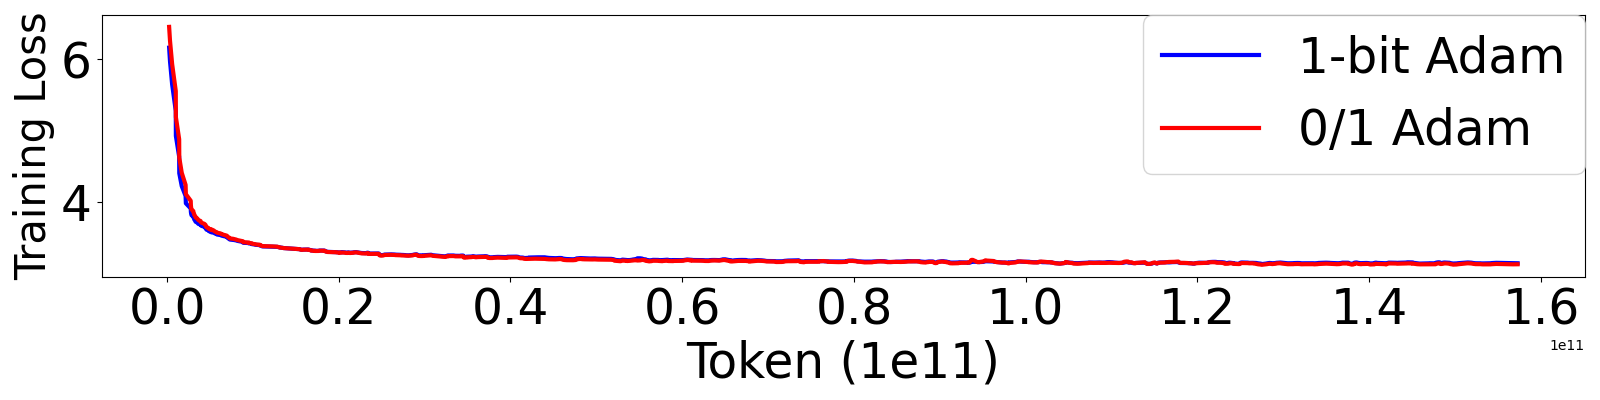
\includegraphics[width=0.49\textwidth]{./sections/figure/v3_gpt2_sample.png}
  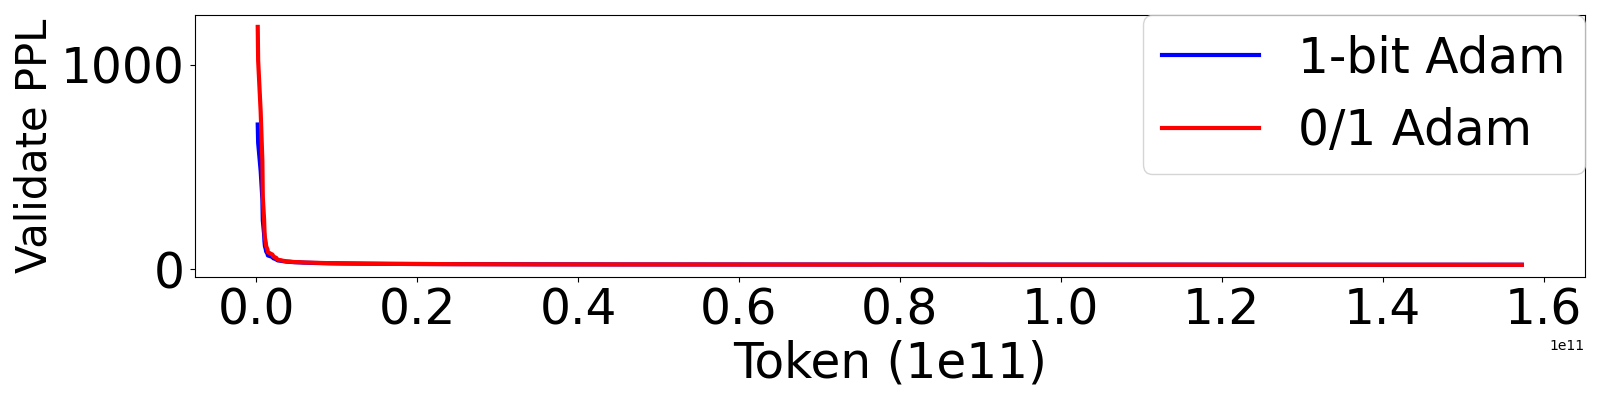
\includegraphics[width=0.49\textwidth]{./sections/figure/v3_gpt2_val.png}
  \caption{Training loss (left) and validation perplexity (right) with respect to Tokens for 1-bit Adam and {\myalgo}.}
  \label{exp:fig:gpt_converge}
\end{figure}

% Figure~\ref{exp:fig:gpt_converge} shows that {\myalgo} is able to achieve the same convergence speed as 1-bit Adam with less communication rounds and bits per parameters, which is aligned with our findings on BERT and ImageNet tasks. Table~\ref{exp:table:gpt} summarizes the quality of output models via zero-shot tasks over WikiText-103 and LAMBADA datasets. We observe {\myalgo} is able to achieve the comparable perplexity and accuracy with Adam, while higher than 1-bit Adam.

% \begin{table}[h!]
%   \centering
%   \caption{Zero-shot evaluation of the trained models on WikiText-103 and LAMBADA datasets, the evaluation methodology follows \citep{shoeybi2019megatron}. The number for Adam is obtained from \citep{li2021curriculum}.}
%   \label{exp:table:gpt}
%   \begin{tabular}{lccccccccc}
%   \hline  
%   & WikiText Perplexity $\downarrow$ & LAMBADA accuracy $\uparrow$ \\
%   \hline 
%   Adam & 27.78 & 33.19 \\
%   1-bit Adam & 28.37 & 33.21 \\
%   {\myalgo} & 28.07 & 33.51 \\
%   \hline
%   \end{tabular}
% \end{table}